% Author: Paul Shao
% Email: paulshaoyuqiao1@berkeley.edu

Living things like you and me inherit from our parents many of their physical characteristics. In the study of population genetics, there are several types of inheritance; one of them is the \textbf{autosomal type}, where each heritable trait is assumed to be governed by a single gene. \\

Typically, there are two different forms of genes denoted by $A$ and $a$. Each individual in a population carries a pair of genes; the pairs are called the individual's genotype. This gives three possible genotypes for each inheritable trait: $AA$, $Aa$, and $aa$ ($aA$ is genetically the same as $Aa$, or in other words, the order of the genes in the genotypes doesn't matter). \\

As some of you might have recalled from a high school biology class, the Mendel's experiment is one of the earliest genetics studies that explores the possible genotypes and variation in the inheritable traits from crossing different individuals in the population:
\begin{figure}[H]
    \centering
    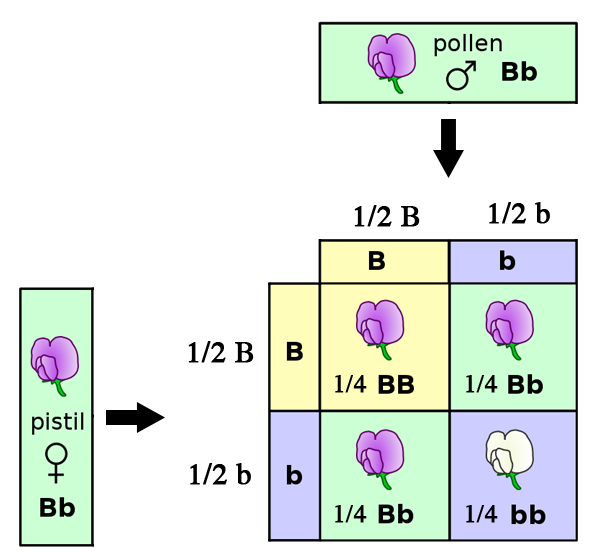
\includegraphics[width=6cm]{../flowers.png}
    \caption*{\textit{Mendel's Experiment using Punnet Square}}
\end{figure}

As you can see in the figure above, each cell in the square represents the chance that you will get a specific genotype for the flower after crossing. \textbf{The reason we care to calculate such chances} is because among the majority purple flowers, you can find a white flower (which fully manifests a recessive trait). Unfortunately, recessive traits will sometimes show in the form of disorders or diseases. Here's an example of how studying the likelihood of genotypes on the genotype that can cause \textit{Cystic Fibrosis} (a very serious neural degenerative disease).
\begin{figure}[H]
    \centering
    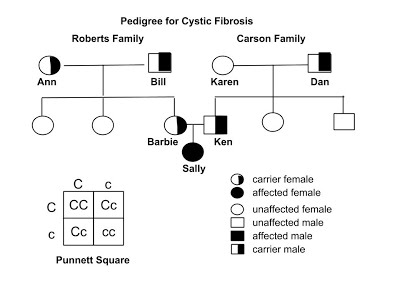
\includegraphics[width=9cm]{../pedigree.png}
\end{figure}
Now that you have some background in how popular genetics works, let's dive back to this problem! Suppose we have just discovered a new population of animals on a hypothetical Planet 16A, and our biologist-in-residence Kevin has found that an autosomal model of inheritance controls eye coloration (what colors the eyes have). Here is what Kevin has found:
\begin{itemize}
    \item Genotypes $AA$ and $Aa$ have brown eyes.
    \item Genotype $aa$ has blue eyes.
\end{itemize}

Kevin believes that the $A$ gene dominates the $a$ gene, and he further classifies an animal as \textbf{dominant} if it carries $AA$ genes, \textbf{hybrid} if it carries $Aa$ genes, and \textbf{recessive} if it carries $aa$ genes. We can see that in this case, the dominant and hybrid genes are indistinguishable in appearance.

To further investigate how the distribution of the eye-color genes of this animal change over time, as a leading engineer on the research team, you are tasked with simulating the distribution of genotypes over multiple generations for this animal.

\textbf{Note: } for all of the following parts, we assume that each offspring inherits one gene from each parent in a completely random manner. 
\begin{enumerate}
    \item Given the genotypes of the parents, we can determine the distribution of the genotypes for the offspring. Suppose that in the original sample of 200 animals, 50 of them carry the \textbf{dominant} genes, 120 of them carry the \textbf{hybrid} genes, and the rest carries the \textbf{recessive} genes. We want to represent this distribution as a vector $\vec{v_p}^{(0)}$, where each entry $v_{p, i}$ in $\vec{v_p}^{(0)}$ represents the chance that a randomly selected animal from our sample population carries the genotype $i$. Find $\vec{v_p}^{(0)}$ (Entries should be in order of \textbf{dominant}, \textbf{hybrid}, and \textbf{recessive})
    
    \note{When explaining this problem, focus on how we can relate the process of choosing an animal randomly and discovering its genotype to the overall proportion of each genotype in the population. It might be a good idea to start with a much smaller number for the sample population so you can actually draw out each genotype in the sample population on the board.} 
    
    \sol{The chance that a randomly selected animal carries the genotype $i$ can be represented by the proportion of the genotype $i$ with respect to the total sample population.
    $$\vec{v_p}^{(0)} = \begin{bmatrix}
50/200\\ 
120/200\\
(200-50-120)/200 

\end{bmatrix} = \begin{bmatrix}
1/4\\ 
3/5\\ 
3/20
\end{bmatrix}$$}

    \item Now, you woud like to consider a series of simulated experiments where we continuously breed all animals in our sample population \textbf{only} with animals that carry a \textbf{dominant} genotype. Suppose after 1 round of breeding, the distribution of the genotypes in our population becomes $\vec{v_p}^{(1)}$. Find $\vec{v_p}^{(1)}$. 
    
    \textbf{Note: } For ease of computation, for all later parts of this question, we will assume that the original distribution vector (for the genome) $$\vec{v_p}^{(0)} =
    \begin{bmatrix}
        Pr(AA \text{ at } t = 0) \\
        Pr(Aa \text{ at } t = 0) \\
        Pr(aa \text{ at } t = 0)
    \end{bmatrix} = \begin{bmatrix}
1/3\\ 
1/3\\
1/3 
\end{bmatrix}$$

    \note{For this question, make sure to explain how gene crossing works for the students: especially the part where an offspring inherits exactly one randomly chosen gene from both of its parents.}
    
    \sol{Let us consider this 1 round of breeding in 3 different scenarios (based on what initial genotype the animal has).
    
    \begin{itemize}
        \item $AA$ with $AA$ (dominant + dominant): Since the offspring will have one gene from each parent, it will be of type $AA$ as well. Thus the probabilities of $AA$, $Aa$, and $aa$ are 1, 0 and 0 respectively.
        \item $Aa$ with $AA$ (hybrid + dominant):  Taking one gene from each parent, we have the possibilities of $AA$, $AA$ (taking $A$ from the first parent and each $A$ in turn from the second parent), $aA$, and $aA$ (taking a from the first parent and each $A$ in turn from the second parent). Thus the probabilities of $AA$, $Aa$, and $aa$, respectively, are 1/2, 1/2 and 0.
        \item $aa$ with $AA$ (recessive + dominant): There is only one possibility, namely $aA$. Thus the probabilities of $AA$, $Aa$, and $aa$ are 0, 1 and 0 respectively.
    \end{itemize}

    For those more comfortable with probability notations, we can rephrase the calculations above as the following: \\ \\
    For each of the genotypes ($AA, Aa, aa$), the respective probability of us getting a particular genotype $T$ (i.e. $T$ could potentially be $AA$, $Aa$, or $aa$) by crossing with a \textbf{dominant} genotype is:
    $$
    \begin{aligned}
        Pr(AA \text{ CROSS } AA \Rightarrow T) &= \frac{Pr(Ti \in \{ A, A \} \times \{A, A \} )}{4} \\
        Pr(Aa \text{ CROSS } AA \Rightarrow T) &= \frac{Pr(Ti \in \{ A, a \} \times \{A, A \} )}{4} \\
        Pr(aa \text{ CROSS } AA \Rightarrow T) &= \frac{Pr(T \in \{ a, a \} \times \{A, A \} )}{4}
    \end{aligned}
    $$
    Here, $ \times $ represents the \textbf{cross product} between 2 sets of elements: it creates a set containing all possible pairwise combinations of the elements from both sets.

    Now that we know the new distribution of genotypes given any one of the initial genotypes (\textbf{dominant}, \textbf{hybrid}, \textbf{recessive}), we can calculate the new overall distributions for the genotypes:
    \begin{itemize}
        \item \textbf{Dominant}: $1(1/3) + 1/2(1/3) + 0(1/3) = 1/2$
        \item \textbf{Hybrid}: $0(1/3) + 1/2(1/3) + 1(1/3) = 1/2$
        \item \textbf{Recessive}: $0(1/3) + 0(1/3) + 0(1/3) = 0$
    \end{itemize}

    Hence, we know that:
    $$\vec{v_p}^{(1)} = \begin{bmatrix}
1/2\\ 
1/2\\
0 
\end{bmatrix}$$
}

\item Now that you have completed one round of breeding with the \textbf{dominant} genotype, you are eager to continue more rounds of simulation. However, before going about doing this, you would like to know if you can re-represent this one round of breeding in a more concise and matrix-oriented way. In other words, you would like to see if there exists a matrix $A$ such that it can predict what the $(T+1)$st (next) round's distribution of genotypes will be given the $T$th (current) round. Mathematically, we can represent this as the equation below:
$$\vec{v_p}^{(T+1)} = A\vec{v_p}^{(T)}$$
Does $A$ exist? If so, find $A$; if not, explain why.

\note{As a great place to start, encourage the students to look through the previous part when we calculated the distribution of genotypes after the first round of breeding. Specifically, motivate the students to look at how the new distribution is calculated individually for each genotype (as a linear combination)}

\sol{Based on the previous part, we can observe how we calculate the distribution of genotypes after the first round of breeding. Specifically, given:
    \begin{itemize}
        \item \textbf{Dominant}: $1(1/3) + 1/2(1/3) + 0(1/3) = 1/2$
        \item \textbf{Hybrid}: $0(1/3) + 1/2(1/3) + 1(1/3) = 1/2$
        \item \textbf{Recessive}: $0(1/3) + 0(1/3) + 0(1/3) = 0$
    \end{itemize}
We can interpret the new distribution of each genotype as follows (here, we use \textbf{dominant} genotype as an example):
The new distribution of the dominant genotype is equal to the sum of all the followings:
\begin{enumerate}
    \item $Pr(AA^{(T+1)} \:|\: AA^{(T)})P(AA^{(T)})$ \\ The probability of a dominant genotype given that the original genotype is also \textbf{dominant} $\times$ the original distribution of the dominant genotype
    \item $Pr(AA^{(T+1)} \:|\: Aa^{(T)})P(Aa^{(T)})$ \\ The probability of a dominant genotype given that the original genotype is \textbf{hybrid} $\times$ the original distribution of the dominant genotype
    \item $Pr(AA^{(T+1)} \:|\: aa^{(T)})P(aa^{(T)})$ \\ The probability of a dominant genotype given that the original genotype is \textbf{recessive} $\times$ the original distribution of the dominant genotype
\end{enumerate}
For those who are interested and familiar with some probability theory, this is \textbf{no more than an application of Bayes' Theorem on conditional probabilities}!
$$
\begin{aligned}
    Pr(AA^{(T + 1)}) \\
    &= \sum_{trait^{(T)} \in \{AA^{(T)}, Aa^{(T)}, aa^{(T)}\}} Pr \left[ AA^{(T+1)}, \: trait^{(T)} \right] \\
    &= \sum_{trait^{(T)} \in \{AA^{(T)}, Aa^{(T)}, aa^{(T)}\}} Pr\left[AA^{(T+1)} \: | \: trait^{(T)}\right] Pr\left[trait^{(T)}\right] \\
    &= Pr\left[AA^{(T+1)} | AA^{(T)} \right]P\left[AA^{(T)}\right] + Pr\left[AA^{(T+1)} | Aa^{(T)} \right]P\left[Aa^{(T)}\right] + Pr\left[AA^{(T+1)} | aa^{(T)} \right]P\left[aa^{(T)}\right]
\end{aligned}
$$
From a matrix-vector multiplication standpoint, we can see that we are actually computing the linear combination of all the respective chances of acquiring a dominant genotype given different initial genotypes with respect to the original genotype (as in the first entry of our distribution vector $\vec{v_p^{(0)}}$). 

Applying the same observations for other vectors, we can deduce our matrix $A$ from the following matrix-vector decomposition:
$$\vec{v_p}^{(1)} = \begin{bmatrix}
1(1/3) + 1/2(1/3) + 0(1/3) \\ 
0(1/3) + 1/2(1/3) + 1(1/3)\\
0(1/3) + 0(1/3) + 0(1/3) 
\end{bmatrix} = 
\begin{bmatrix}
\frac{1}{3}
\begin{bmatrix}
1\\ 
0\\ 
0
\end{bmatrix} & \frac{1}{3}
\begin{bmatrix}
1/2\\ 
1/2\\ 
0
\end{bmatrix} & \frac{1}{3}
\begin{bmatrix}
0\\ 
1\\ 
0
\end{bmatrix}
\end{bmatrix} = \begin{bmatrix}
1 & 1/2 & 0 \\ 
0 & 1/2 & 1\\
0 & 0 & 0
\end{bmatrix}\begin{bmatrix}
1/3\\ 
1/3\\ 
1/3
\end{bmatrix} = A\vec{v_p}^{(0)}$$
Therefore, we can see that:
$$A = \begin{bmatrix}
1 & 1/2 & 0 \\ 
0 & 1/2 & 1\\
0 & 0 & 0
\end{bmatrix}$$
}

\item \textbf{Without explicitly solving for the inverse or row reducing the matrix}, determine if the transformation matrix $A$ is invertible or not. Provide your explanations in a few sentences. 

\note{Encourage the students to think in the context of the question, specifically on the previous example of how one round of breeding is done and what happens to the distribution of each genotype. It might be helpful to point out to students that the distribution of the receissive traits comes from the bottom row of $A$.}

\sol{$A$ is not invertible. We can tell this by looking at specifically the breeding of an initially \textbf{recessive} genotype ($aa$) with the \textbf{dominant} ($AA$) genotype. Over 1 round of breeding, the new distribution of $aa$ has dropped to 0, meaning that it no longer exists in our distribution. In a geometric way, we can interpret this as we have "collapsed" one dimension of the distribution vector. From an invertibility standpoint, given the current distribution of genomes, where there are 0 recessive genotypes, it is \textbf{impossible} for us to actually tell what the distribution for the recessive genotypes from the previous round will be (since everything is dropped to 0 regardless). Since we cannot determine what the previous distribution is given the current one, we cannot find the inverse of $A$, and thereby, $A$ is not invertible.}


\end{enumerate}

